\documentclass[tikz,border=8pt]{standalone}
% Shared look for every TikZ diagram. Load with \input{../../tools/tikz-style.tex}
\usepackage[sfdefault]{roboto}
\usetikzlibrary{arrows.meta, positioning, shapes.geometric, calc, fit, backgrounds}
\definecolor{cblue}{HTML}{4C78A8}
\definecolor{corange}{HTML}{F58518}
\definecolor{cgreen}{HTML}{54A24B}
\definecolor{cred}{HTML}{E45756}
\definecolor{cpurple}{HTML}{B279A2}
\definecolor{cgrey}{HTML}{6B6B6B}
\tikzset{
  every picture/.style={font=\sffamily, line width=1.2pt},
  box/.style={draw=#1, fill=#1!12, rounded corners=4pt, align=center, inner sep=7pt, minimum height=1.1cm},
  box/.default=cgrey,
  arrow/.style={-{Stealth[length=3mm]}, draw=cgrey, line width=1.4pt},
  title/.style={font=\sffamily\bfseries\Large},
  note/.style={font=\sffamily\small, text=cgrey, align=center},
}
\AtBeginDocument{\hyphenpenalty=10000 \exhyphenpenalty=10000}

% One program, two robots: the same controller node read with two parameter files. Nav2's default
% (nav2_bringup/params/nav2_params.yaml, main): controller_frequency 20.0, FollowPath vx_max 0.5. Ours: 0.6 m/s,
% the room robot's top forward speed (both wheels at 0.6 m/s).
\begin{document}
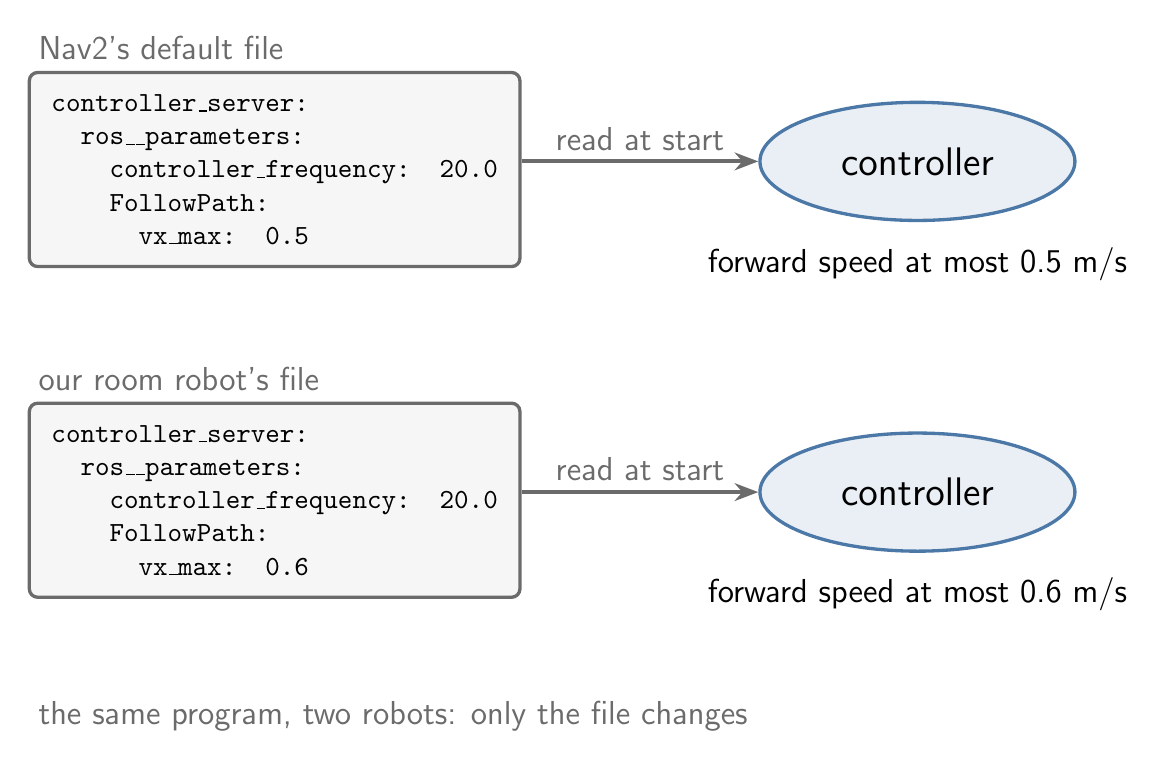
\begin{tikzpicture}[
  y1/.style={draw=cgrey, fill=cgrey!6, rounded corners=3pt, font=\ttfamily\normalsize, align=left, inner sep=8pt, anchor=north west},
  nd/.style={draw=cblue, fill=cblue!12, ellipse, font=\sffamily\Large, inner sep=6pt, minimum width=4cm, minimum height=1.5cm}]
  \node[y1] (a) at (0,0) {controller\_server:\\ \ \ ros\_\_parameters:\\ \ \ \ \ controller\_frequency: 20.0\\ \ \ \ \ FollowPath:\\ \ \ \ \ \ \ vx\_max: 0.5};
  \node[y1] (b) at (0,-4.2) {controller\_server:\\ \ \ ros\_\_parameters:\\ \ \ \ \ controller\_frequency: 20.0\\ \ \ \ \ FollowPath:\\ \ \ \ \ \ \ vx\_max: 0.6};
  \node[note, font=\sffamily\large, anchor=south west] at (a.north west) {Nav2's default file};
  \node[note, font=\sffamily\large, anchor=south west] at (b.north west) {our room robot's file};
  \node[nd] (n1) at (11.3,-1.15) {controller};
  \node[nd] (n2) at (11.3,-5.35) {controller};
  \draw[arrow] (a.east |- n1) -- node[note, above, font=\sffamily\large] {read at start} (n1);
  \draw[arrow] (b.east |- n2) -- node[note, above, font=\sffamily\large] {read at start} (n2);
  \node[note, font=\sffamily\large, text=black] at (11.3,-2.45) {forward speed at most 0.5 m/s};
  \node[note, font=\sffamily\large, text=black] at (11.3,-6.65) {forward speed at most 0.6 m/s};
  \node[note, font=\sffamily\large, align=left, anchor=west] at (0,-8.2) {the same program, two robots: only the file changes};
\end{tikzpicture}
\end{document}
